\documentclass[12pt]{article}                       % Make it an article
\usepackage{indentfirst}                            % All subsections indented
\usepackage{setspace}                               % For 1.5 spacing
\usepackage{hyperref}                               % Make table of contents clickable, allow URLs
\usepackage[letterpaper, margin=1in]{geometry}      % 1 inch margin, letter paper (American)
\usepackage[english]{babel}                         % For "fancy" quotes
\usepackage[autostyle, english=american]{csquotes}  % Same
\usepackage{apacite}                                % Use APA citations
\usepackage{etoolbox}                               % Misc
\usepackage{titlesec}                               % Modify spacing
\usepackage{listofauthorships}                      % CUSTOM BUILT (lifted from S/O)! Adds a table of authorship
\MakeOuterQuote{"}                                  % For fancy quotes
\usepackage{times}                                  % For tilde
\usepackage{textcomp}                               % For tilde
\usepackage{graphicx}                               % Images
\usepackage{array}                                  % Table spacing
\usepackage{ragged2e}                               % Left align table text
\usepackage{float}                                  % Image placement
\usepackage{longtable}                              % Long tables

% Document-level options
\hypersetup{colorlinks=true,
            urlcolor=blue,
            citecolor=black,
            linkcolor=black}
\titlespacing*{\section}{0pt}{0pt}{0pt}
\titlespacing*{\paragraph}{12pt}{0pt}{6pt}
\titlespacing*{\subsection}{0pt}{5pt}{-5pt}
\titlespacing*{\subsubsection}{0pt}{5pt}{-3pt}

% Set up document title info
\title{Eilat: Transportation 2040}
\author{Evan Goldstein, Valeria Kopper, Christopher Myers, Zachary Zlotnick}
\date{\today}

\begin{document}

% Title page
\pagenumbering{gobble}
\maketitle
\vspace{12cm}
\begin{minipage}{0.5\textwidth}
    \begin{flushleft} \large
        
\includegraphics[width=2.5cm]{images/eilat_logo.png} \\
        \textbf{Sponsored by:} \\
        A. Adamon, \\
        E. Toppel \\
        \textit{Eilat Municipality}
    \end{flushleft}
\end{minipage}
~
\begin{minipage}{0.4\textwidth}
    \begin{flushright} \large
        
\includegraphics[width=5.5cm]{images/WPI_logo.png} \\
        \vspace{0.7cm}
        \textbf{Submitted to:}\\
        Professor Bar-On
        \vspace{1.5cm}
    \end{flushright}
\end{minipage}

\newpage

\renewcommand\abstractname{Summary} % "Abstract" -> "Summary", the header lies

\pagenumbering{roman}
\tableofcontents
\vspace{1cm}
\listoffigures \newpage
\listofauthorships
\pagenumbering{arabic}
\doublespacing

% Actual content begins here!
\section{Introduction}[All]
Eilat is a city in the southern tip of Israel with a growing population of ~50,000 and an area of 85 km$^2$. The city is a popular tourist destination, with over 3 million tourists per year from around the world. Given past trends, tourism is expected to continue increasing in the future. The city currently suffers from heavy congestion at peak hours, and the new Ramon airport on route 90 is expected to worsen the situation, increasing travel times. This compounded congestion will put a strain on Eilat's transport network, calling for an increased effort to shorten commute times, expand Eilat's transportation services, and streamline the travel experience. 

Currently, Eilat's public transport offerings are limited to taxis and intra-city buses operated by Egged. A bus ride from the west side of the city to the airport takes about 26 minutes with no traffic, and from Yotam Square to the Hotels zone is 35 minutes. These lengthy travel times are likely due to a high number of stops across a wide area. Strategically implemented policy changes, city restructuring, and connected technologies are proven to increase city efficiency.

Eilat's growing population and fluctuating tourism throughout the year have both placed strain on the existing transportation network, leading to heavy congestion. This project aimed to determine goals for Eilat's future transportation services that have successfully tackled by making use of smart city technologies. We worked to identify the gap between these cities' transportation network and Eilat's, to assist in better designing and allocating mobility services throughout the city. As part of that work we created a roadmap to serve as a guide that includes a goal-oriented timeline, and an interactive website with maps and air traffic data to assist city planners and inform them on the results of our work.
 
\newpage
\section{Background --- Eilat's Current Situation }
Despite Eilat's population of only fifty thousand, its situation is complicated by congestion, the inefficiencies of the bus system, the influx of three million tourists every year, and future expansion plans.

\subsection{Existing Transportation}
\subsubsection{Congestion}[C.M.]

\begin{figure}[H]
    \centering
    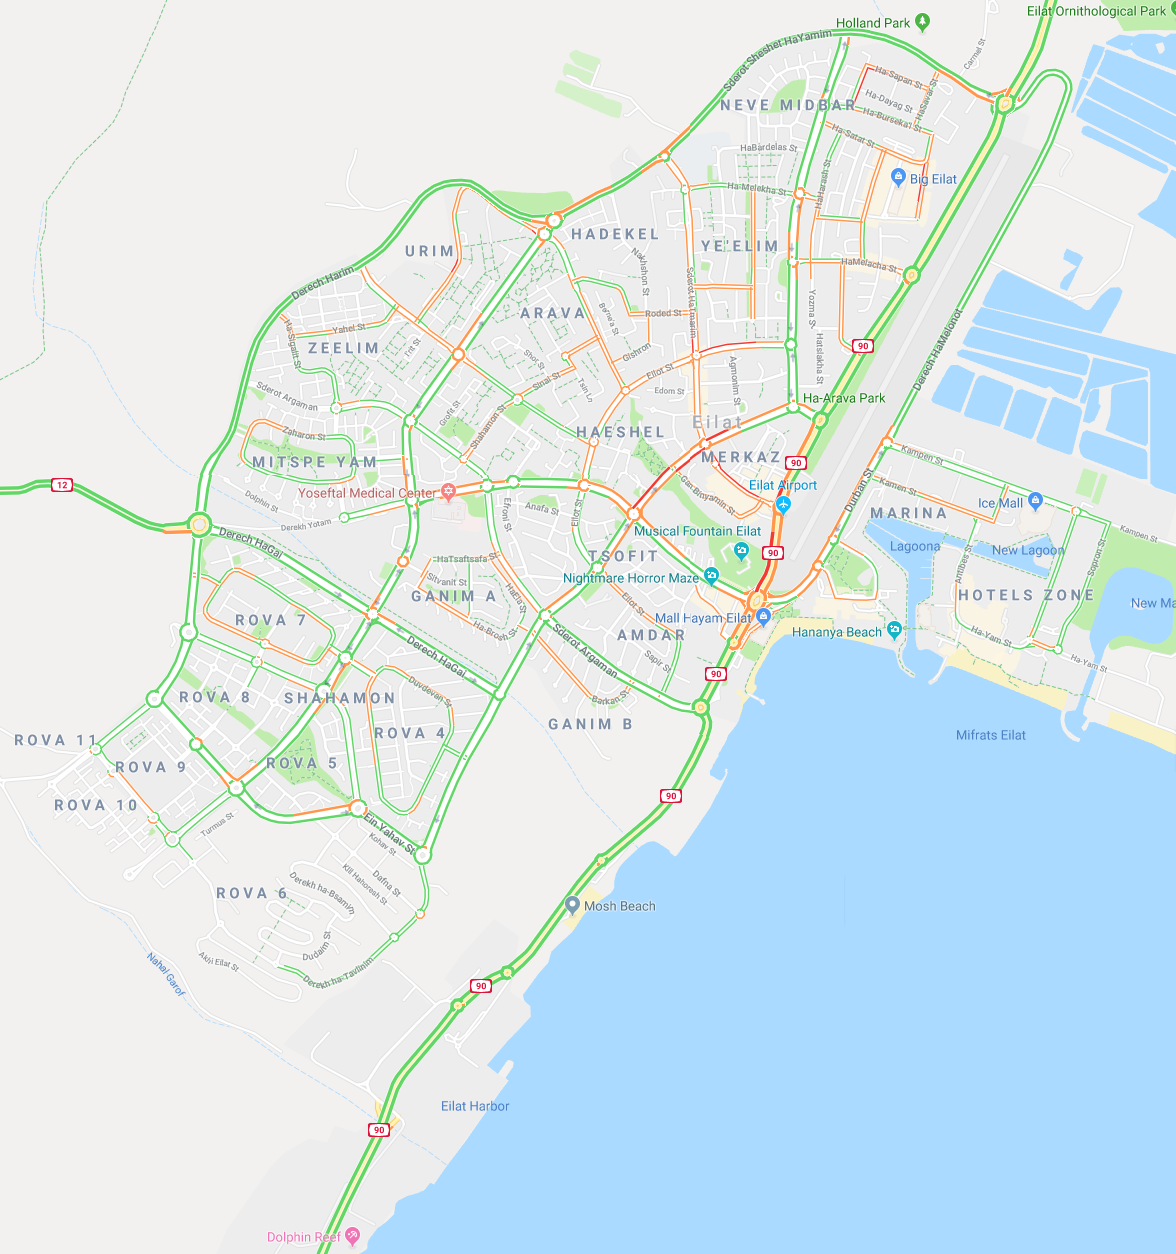
\includegraphics[scale=1]{images/eilat_traffic.png}
    \caption{Traffic map of Eilat at 5 PM weekdays (off-season)}
    \label{img:eilatTraffic}
\end{figure}

Israel's route 90 is the main road leading into Eilat, seen in the top right of figure \ref{img:eilatTraffic}, and is subject to heavy congestion during the tourism season, especially during peak hours. Red and orange roads indicate heavy and moderate congestion, respectively. During rush hours congestion is moderate in most major city arteries, even off-season. A notable hotspot is the Eilat airport (on the center right) which travelers frequently enter and exit. However, this airport is set to shut down as Ramon Airport along route 90 sees more traffic, and Ovda Airport (which feeds into route 12 on the far left) will stop handling civilian flights. This leaves Ramon airport as the only airport servicing Eilat, enhancing the already-present focal point for congestion wherever route 90 meets with city roads. Commuting times see residents crowd on three major roads in the residential zone to the west as they move east to the industrial and commercial sectors of the city. The fact that three of Eilat's major schools are located along these roads only worsens congestion as parents drop off and pick up their children. Given current congestion, major traffic jams and long travel times can only be expected to increase.

\subsubsection{Bus System}[E.G.]
Currently, Egged operates intra-city buses in Eilat. A bus ride across the city from the west to the hotel zone in the east takes between thirty and thirty five minutes, while the same journey by car takes ten. Lengthy bus travel times are due to a high number of stops across a wide area for any given route. Despite launching twenty-five electric buses in Haifa in 2017, the Egged fleet still consists almost entirely of diesel-powered buses. Diesel powered vehicles do not fit with Eilat's desire to reduce its ecological impact.

%Bus stops are highly concentrated in residential areas, and frequently in close proximity to one another (often as close as 50 meters). City-wide, there is almost always at least one bus stop within a 5 minute walking distance. Often, buses do not arrive at a given stop frequently, and a choice must be made between a longer wait and a longer walk.

%add info about actual usage and routes

Moovit is the most popular public transportation app, and provides information about expected arrival times of buses at a given stop in real time. Without the use of Moovit, it is difficult to predict when a bus will arrive at a stop. The app can only display Israel' bus information in Hebrew, making it difficult for international tourists to use.

\subsection{Tourism}
\subsubsection{Statistics}[Z.Z.]
Domestic tourism is a major part of Israel's tourism industry, accounting for 90\% of hotel room occupation in Eilat \cite{Benner2017UpgradingEilat}. The Ministry of Tourism spends approximately 33\% of its budget on marketing, 28\% on investment incentives, and 26\% on infrastructure investment \cite{Benner2017UpgradingEilat}. The United States, Russia, France, the UK, and Germany account for nearly 50\% of international tourists. In 2012 Israel attempted to draw in more European and American tourists through an agreement with the European Union (EU) to allow direct flights between Israel and all EU countries \cite{Benner2017UpgradingEilat}. This agreement, called Open Skies, drove flight prices down and increased tourist flow to all parts of Israel. As of 2015, France and Russia represented the largest origin markets with a 42\% and 26\% claim respectively on international tourist arrivals Eilat, suggesting that Open Skies increased tourism pull from the EU. \cite{Benevolo2016SmartBenefits}.

\subsubsection{Demographics}[V.K.]
In 2018 there were a total of about 6.5 million overnight tourists, of which approximately 89\% were Israeli tourists according to our sponsor. In 2018, hotel occupation was 73.2\%, or 11,034 hotel rooms.

A clear majority of tourism in Eilat is domestic. With the average from 2000 to 2018 showing a majority of 87\% of tourism accounted by Israelis and the remaining 13\% is international tourism. 

Figure \ref{img:israeli_overnight_tourism} shows a steady, slight increase in domestic overnight tourism from 2000 to 2018.
\begin{figure}[H]
    \centering
    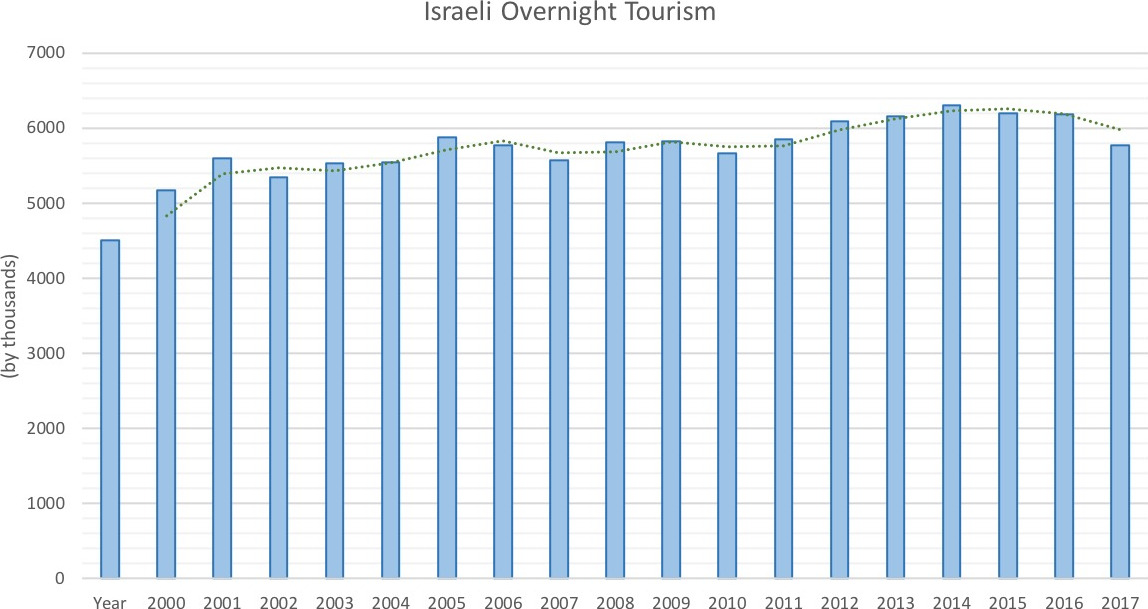
\includegraphics[width=12cm]{images/israeli_overnight_tourism.jpg}
    \caption{Israeli overnight tourism over time}
    \label{img:israeli_overnight_tourism}
\end{figure}

Figure \ref{img:international_overnight_tourism} displays varying international overnight tourism from 2000 to 2018.
\begin{figure}[H]
    \centering
    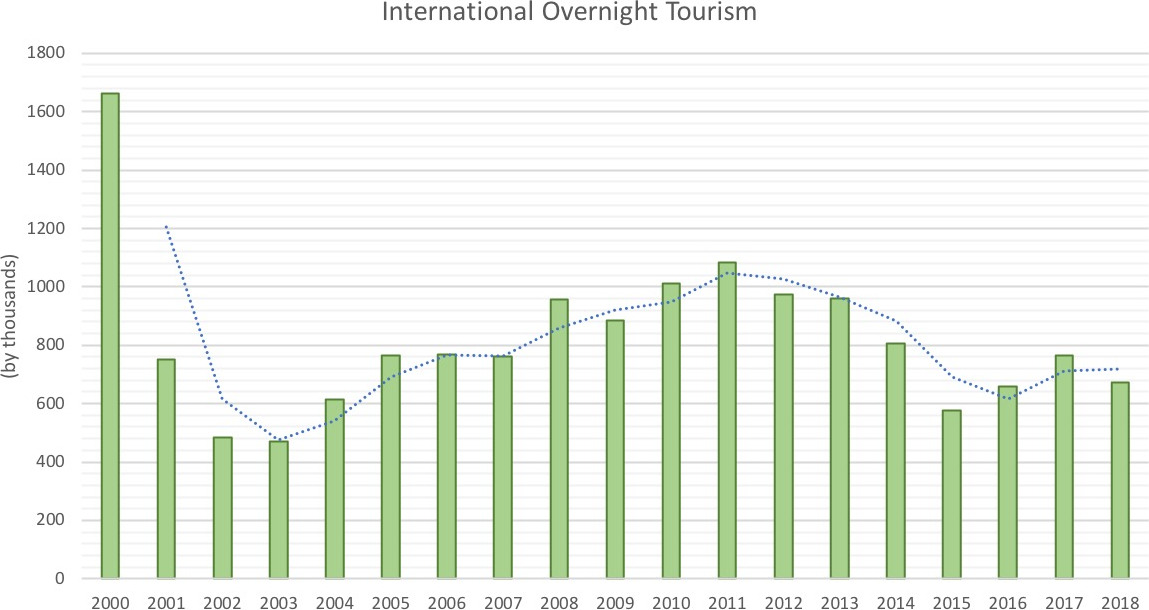
\includegraphics[width=12cm]{images/international_overnight_tourism.jpeg}
    \caption{International overnight tourism over time}
    \label{img:international_overnight_tourism}
\end{figure}

\subsubsection{Popular attractions}[Z.Z.]
Eilat's Red Sea beaches, coral reefs and marine life provide plenty of diving and snorkeling opportunities for tourists \cite{Benner2017UpgradingEilat}. The underwater observatory pulls people from all over and provides views of sharks, turtles, and rare fish (cite min of tourism). The musical fountain is a popular nighttime attraction, offering a unique audiovisual show to pair with the view of the city behind it. As a tax-free city Eilat is a major shopping center with five shopping malls within one square kilometer, the largest being Mall Hayam and the Ice Park Mall \cite{Benner2017UpgradingEilat}. These sites best serve families with children as they provide attractions for all ages and demographics. The city night life, including restaurants, bars, and clubs, makes it well-suited to young adults.

\subsection{Expansion and Zoning}[V.K., Z.Z.]

Figure \ref{img:eilat_zoning} shows Eilat's current layout and how it is zoned into residential, industrial, commercial and tourist areas. 

\begin{figure}[H]
    \centering
    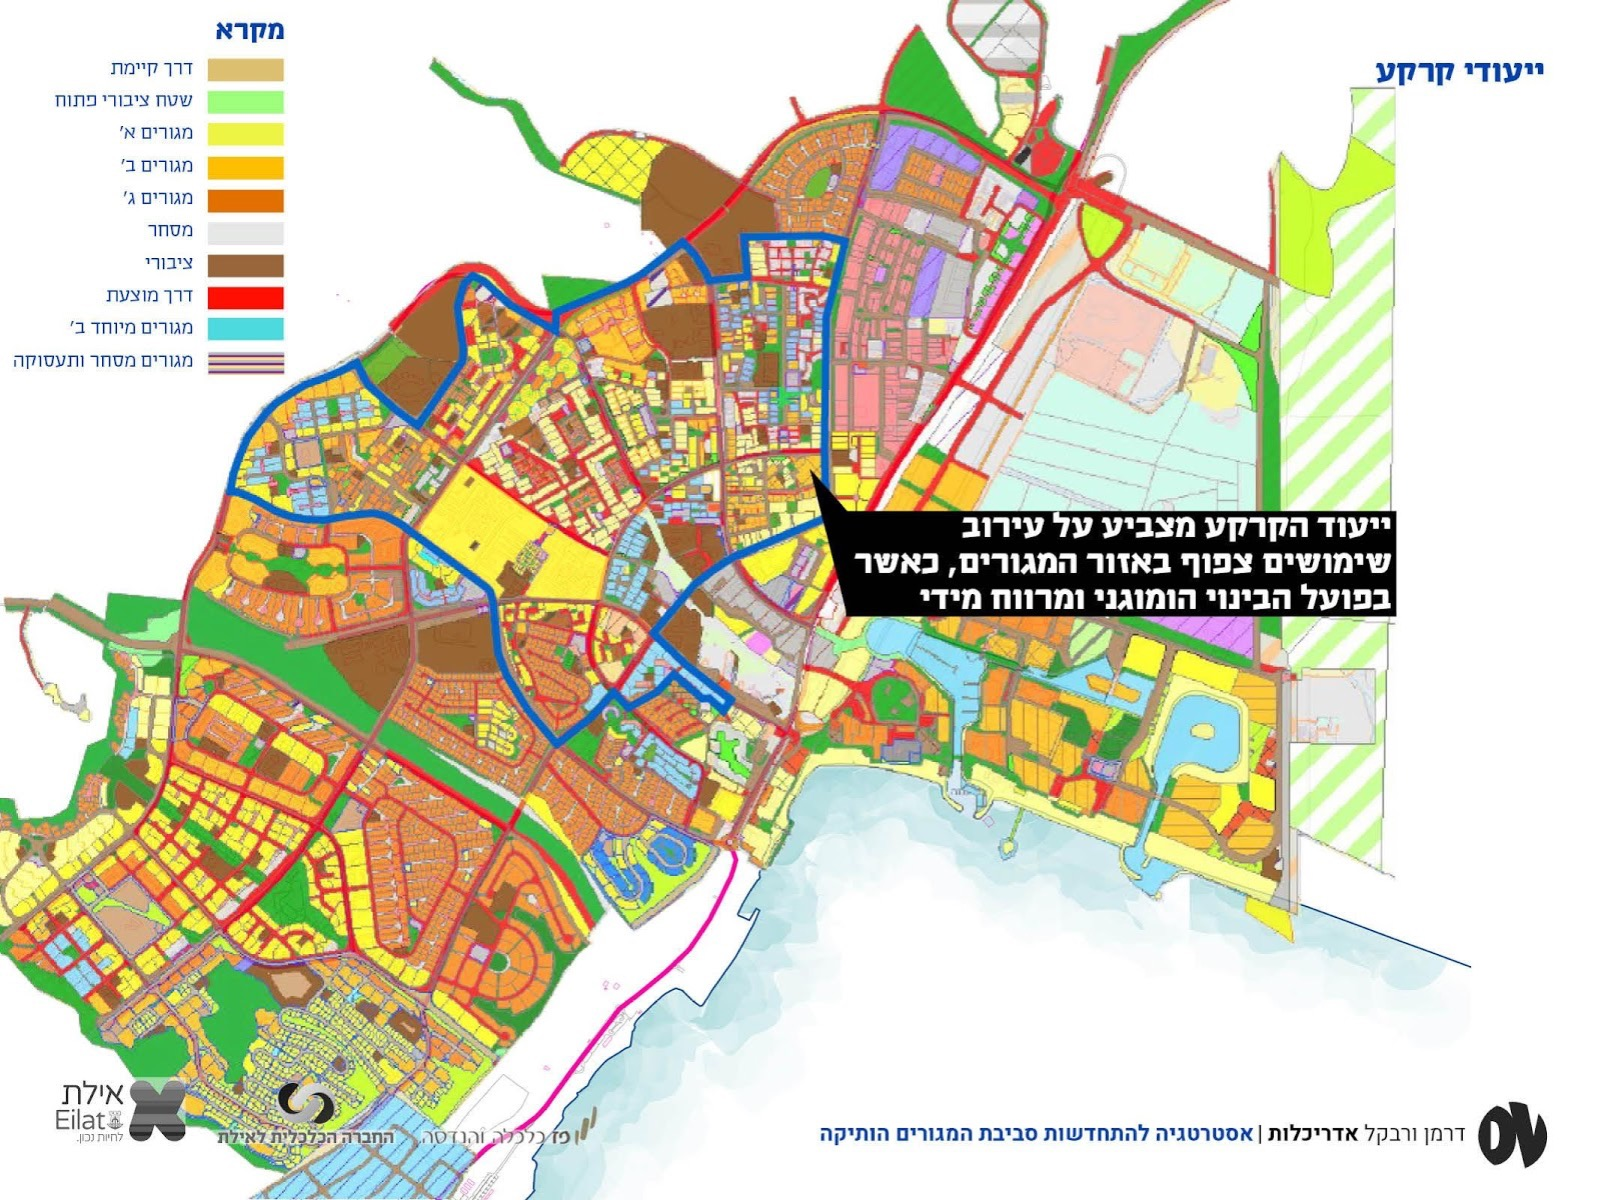
\includegraphics[width=12cm]{images/eilat_zoning.jpg}
    \caption{Map of Eilat zoning}
    \label{img:eilat_zoning}
\end{figure}
Figure \ref{img:eilat_expansion} shows future expansion plans for the city.

\begin{figure}[H]
    \centering
    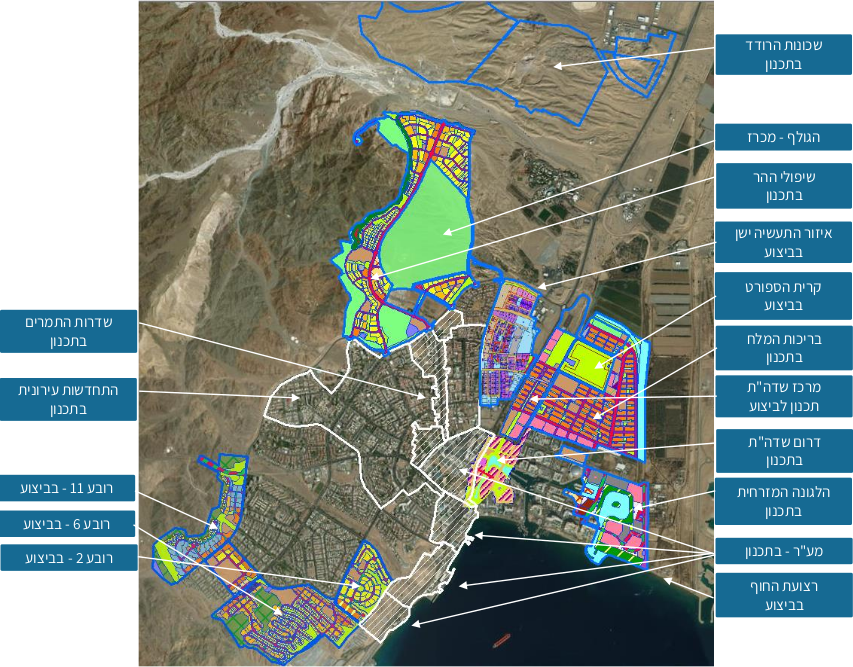
\includegraphics[width=12cm]{images/eilat_zoning_future.png}
    \caption{Map of future Eilat expansion \& zoning}
    \label{img:eilat_expansion}
\end{figure}

Eilat plans to expand the city significantly by adding residences, hotels, and more tourist attractions, including a golf course to the north. These additions will replace the existing airport in the city center, and currently unoccupied land toward the north and south-west. Removing the Eilat Airport will benefit the city, as the airport currently divides parts of the city and increases congestion in the Mall Hayam and Boardwalk area. This expansion would also alleviate some of the congestion that can be seen at peak airport arrival hours when taxis flood the area waiting to pick up travelers. Residents commuting to and from work during airport hours will face less traffic as a result, and services will concentrate toward the north. 

\newpage
\section{Smart Cities}
\subsection{Overview}[V.K., Z.Z.]
Smart cities aim  to ease the lives of their citizens by providing efficient and convenient services, in part by analyzing data collected from sensors throughout the city. Cost, travel time, convenience, reliability, familiarity, weather, safety, environmental considerations, and existing infrastructure are factors that vary across cities and play a crucial role in understanding what citizens and visitors need and want \cite{2016LiveChallenge}. This information can then be used to determine which services should be prioritized.

Existing smart city plans typically first incorporate a basic infrastructure of sensors, cameras, and city-wide WiFi in order to establish a constant stream of data. This data can be used in strategic ways to resolve the issues that are too dynamic and intricate to change via technology-neutral methods. These tools are installed through the city and collect data on traffic, available parking, pedestrian traffic, etc. This information can be used, for example, to improve traffic flow by adjusting public transportation and traffic lights to real-time demand.

Successful smart cities across the world have several common factors, such strong commitments from government leaders that foster collaboration between the public sector and the private sector. Government transparency also greatly increases citizens' confidence and can be achieved by making collected data available. Additionally, prioritizing continuous improvement is crucial due to rapidly changing technologies, since smart cities need to be constantly evolving and adapting alongside them \cite{Zanghi2017WhyExamples}. 

Smart mobility (or mobility as a service) incentivizes customers with cheaper, faster, and more convenient modes of transportation than privately-owned vehicles. These services target issues associated with the saturation of private vehicles, such as traffic congestion, road accidents, insufficient parking, and greenhouse gas emissions.

\subsection{City Case Studies}[V.K]
Detailed below are six examples of cities worldwide that addressed problems such as congestion and pollution. Influencing factors such as population, population density, climate, existing infrastructure, policy flexibility, and public opinion should be taken into account when considering proposed plans. Each city also established different goals, leading to various solutions and implementations. Studying these models provides valuable input for a model reflecting the services and transportation systems needed in Eilat.

\subsubsection{Curitiba, Brazil}[V.K.]
Curitiba is the capital of the state of Paraná in southern Brazil. With 1.8 million people, it is Brazil's 8\textsuperscript{th} most populous city, with about 2 million tourists per year \cite{Adler2016StoryCapital}. During the 1970s there were a series of projects that focused on improving the city after it experienced rapid growth leading to overly congested streets, led by architect and three time mayor Jaime Lerner. The first project, in 1972, converted the main street in the center of the city to a pedestrian mall. The public initially objected to this, especially shopkeepers. To bypass this, Lerner started construction on a Friday evening after the courts had closed and finished within seventy-two hours. Public opinion rapidly shifted when people saw the benefits, instead favored expanding the zone. This was the beginning of an attitude change for Curitiba that focused on bringing people together. Lerner adopted a philosophy of "act now, adjust later" to avoid Brazil's bureaucracy, allowing the implementation of bold initiatives that would otherwise have been shut down or taken longer to carry out. Today, 85\% of the population uses the bus system, given that it is the fastest and cheapest mode of transportation in the city \cite{Adler2016StoryCapital}. The system, known as the Bus Rapid Transit (BRT), uses raised platforms and electronic prepayment that allows for quicker stops, features higher-capacity buses, and has five express bus avenues. The city has made an effort to have large green areas and has a widely adopted recycling program. Curitiba's successful implementation of its bold initiatives has brought it worldwide recognition as a model for urban planning.

\subsubsection{Freiburg, Germany}[Z.Z.]
Freiburg, a city of about 220,000, suffered significant damage during World War II bombings, which led to a redevelopment of the inner areas during the reconstruction period. The population at the time prioritized their energy consumption and city layout, suggesting that a viable solution would focus on city access rather than private vehicles \cite{Rydningen2017OsloCentre}. Planners also decided to place emphasis on supporting diverse, cheap, and clean transportation modes and services \cite{Bindra2006SmartGermany}. Planners also considered air pollution due to traffic in the city center, and pedestrianized the center further to reduce the cars inside. This city center became a hotspot for tourists containing restaurants, shops, and plenty of green space. Parking is available outside the city center at a fee that increases progressively toward the center, reducing congestion \cite{Bindra2006SmartGermany}. The city first ensured there was an efficient tram system, that combined with the bus system was able to bring travelers within 7 minutes of city outskirts. The city also made an effort to expand its biking network by placing bikes next to tram \& bus stations with parking available for cars \cite{Bindra2006SmartGermany}. From 1984 to 2006, public transit use doubled and a 9\% decrease of private vehicle usage for everyday travel needs indicated a modal shift. By 2020, Freiburg is projected to have 29\% of travelers using private vehicles, 20\% using public transit, 27\% using bicylces, with the remaining 24\% walking \cite{Rydningen2017OsloCentre}. Reducing the stress on any one form of transportation should contribute to a well-balanced city-wide network for all users. Figure \ref{img:freiburg_modal_split} reflects the current and projected usage of the transportation network in Freiburg.

\begin{figure}[H]
    \centering
    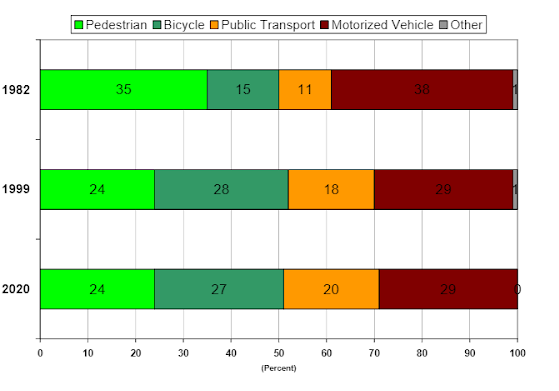
\includegraphics[width=10cm]{images/freiburg_modal_split.png}
    \caption{Chart of Freiburg's transportation modal split over time.}
    \label{img:freiburg_modal_split}
\end{figure}

\subsubsection{Barcelona, Spain}[V.K.]
Barcelona is the second largest city in Spain with 1.7 million residents, and is one of the most densely populated European cities \cite{Bausells2016SuperblocksResidents}. It a popular tourist destination in Europe, with about 8.2 million international visitors per year \cite{Bausells2016SuperblocksResidents}. Barcelona is widely recognized for its smart city initiatives. The city has successfully implemented various smart city technologies, such as sensors that measure air quality, street lights that dim when there are no pedestrians in the area, and sensors in public parks to decrease unnecessary water usage. Parking availability data is also collected through sensors and displayed in a smart parking app that also allows for online payment. The city boasts a smart bus system with increased routes and with smart bus stops that include free WiFi, charging stations and real life time updates of the bus schedule. It has an extensive bike-sharing program with about 180 km of bicycle lanes. The city has a metro system that is 1.5 km per hour faster than the average car trip within the city \cite{Bausells2016SuperblocksResidents}. In order to decrease air pollution, Barcelona will ban cars made before 1997, and trucks \& vans made before 1994. Additionally, Barcelona is now implementing a plan to establish "superblocks" through out the city. These are areas that encompass about nine blocks and prioritize pedestrians. Cars can circulate within the superblocks, but they have to do so at slow speeds, which will ideally lead to cars staying mostly within main roads. Overall, the superblocks aim to foster communities and increase life quality. Figure \ref{img:barcelona_superblock} shows a comparison of the current city layout and the proposed layout structure of superblocks.

\begin{figure}[H]
    \centering
    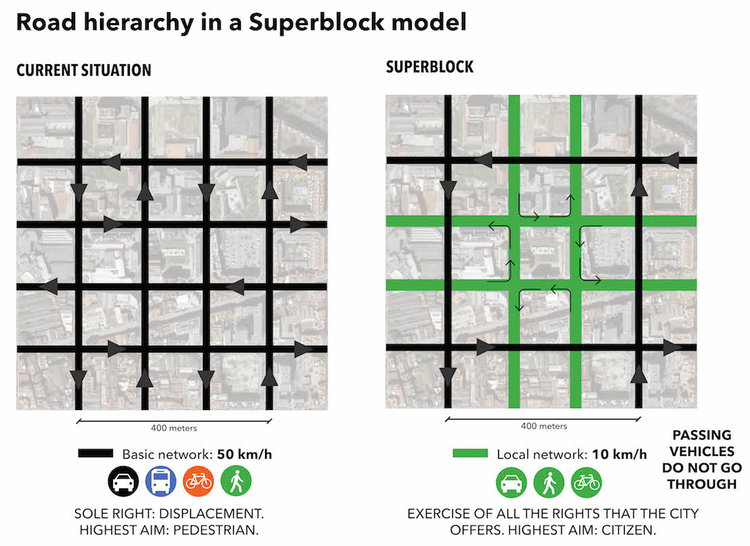
\includegraphics[scale=4.5]{images/barcelona_superblock.jpg}
    \caption{Diagram of Barcelona's "superblocks"}
    \label{img:barcelona_superblock}
\end{figure}

\subsubsection{Kansas City, United States}[Z.Z.]
The Smart City Challenge asked mid-sized cities across the United States to provide a plan for moving to a brand-new transportation system that would "use data, applications, and technology to help people and goods move more quickly, cheaply, and efficiently" \cite{2016BeyondChallengeb}. Kansas City had realistic objectives to create a higher quality of life, reduce traffic, through interconnected smart technologies. At the time of the challenge, having the most highway miles in the region and the most established infrastructure of fiber optics and WiFi in the country was one of Kansas City's most valuable assets. These resources eliminated the need to build a network from scratch, unlike many other cities. The city also emphasized the use of bikes by implementing road diets and including a way-finding app for bikers called RideKC. Though this was a start, Kansas City had 3 different plans in their Smart City + Connected City proposal. Their plan entailed making improvements to underdeveloped areas in the east side, introducing autonomous and connected vehicle technologies, as well as increasing connectivity sharing throughout the city. To address the east side, they added a 3.5 km tram line which allowed easier transport to the center and east side. They also added new way-finding apps for pedestrians, and planned to increase their offerings for ride-sharing and bike-sharing. In addition they began pilot tests for autonomous vehicles in a main artery within the city to test the viability of it expanding. These vehicles will also be connected to events, traffic, and could be implemented slowly while the infrastructure and policy-making develops. The city also plans to partner with cellular and ridesharing companies to obtain important real-time data, further expand the WiFi network to gather user data, and install information kiosks for travelers \cite{2016BeyondChallengeb}.

\subsubsection{Singapore}[Z.Z.]
Singapore has a population of 5.6 million, or nearly 8,000 people per square kilometer, and is expected to grow to 6.9 million by 2030 \cite{2016SmartSingapore}. The city believes it can use its technology-based economy and infrastructure to its advantage to combat the anticipated increase in density. First, the city will make itself more pedestrian and biker-friendly by providing more bike lanes and pedestrian mobility services. Using autonomous cars, the city hopes to implement Mobility as a Service (MaaS) and reduce the amount of private vehicles on the road \cite{Huiling2017AISingapore}. Though autonomous cars are difficult to test in a place with such a significant population density, it would alleviate major congestion areas and reduce accidents, commute times, and allow for vehicle-to-vehicle (V2V) communications. Data gathered from these autonomous vehicles, cameras, sensors, and people on the city-wide network will be analyzed and redistributed to vehicles and travelers to adjust to real-time issues within the city \cite{2016SmartSingapore}. This system would save people money, time, and would make it easier for users to pay. Since vehicles take up 12\% of the city's area, we can assume that constantly moving autonomous cars would significantly increase the amount of available city land previously held by parked private vehicles \cite{Huiling2017AISingapore}. Though Singapore has lofty goals, they hope to achieve full autonomous fleets in the next 10 to 15 years.

\subsubsection{Columbus, United States}[V.K.]
In 2015 Columbus, Ohio won the Smart City Challenge created by the U.S. Department of Transportation (DOT), which resulted in a \$50 million grant given to fund the city's plans to create a smart transportation system \cite{2016ColumbusChallenge}. The city raised an additional \$500 million from mostly the private sector to support further smart technologies, such as funding autonomous vehicle testing. The collaboration between the public and private sectors has been crucial in Columbus's success in implementing its plan to transition into a smart city. It has installed sensors throughout the city that work to allow integrated data exchange (IDE) in order to decrease congestion and smooth transportation. For example, this allows emergency vehicles to interact with traffic lights to decrease travel time. Columbus aims to convert to EVs and wants to decarbonize the city's electric grid. It is also testing autonomous vehicles and created a playbook in order to share projects, case studies, and strategies with other cities looking to implement smart city technologies.

\newpage
\subsubsection{Table of Cities}[V.K., Z.Z.]
\begin{table}[H]
    \centering
    \singlespacing
    \small
    \begin{tabular}{ m{1.7cm} | m{1.1cm} | m{1.3cm} | m{3.4cm} | m{3.4cm} | m{3.4cm} }
        \textbf{City} & \textbf{Pop.} & \textbf{Area} & \textbf{Problem} & \textbf{Goal} & \textbf{Plan} \\
        \hline{}
        Curitiba, Brazil &
        1.76M &
        432km$^2$ &
        \begin{flushleft}Rapid population growth led to high congestion \end{flushleft} &
        \begin{flushleft}Provide better quality of life and transportation for citizens\end{flushleft} &
        \begin{flushleft}Pedestrian city center, bus rapid transportation, biking lanes, and green areas\end{flushleft} \\ 
        \hline{}
        
        Freiburg, Germany &
        227K &
        153km$^2$ &
        \begin{flushleft}Reconstruction after WWII \end{flushleft} &
        \begin{flushleft}Move away from car predominance, prioritize pedestrians\end{flushleft} &
        \begin{flushleft}Pedestrian city center, extend \& improve bike network, expand tram \& bus lines\end{flushleft} \\
        \hline{}
        
        Barcelona, Spain &
        1.6M &
        102km$^2$ &
        \begin{flushleft}High noise \& air pollution, saturated streets\end{flushleft} &
        \begin{flushleft}Move away from car predomincance, prioritize pedestrians\end{flushleft} &
        \begin{flushleft}Mini-superblocks, repurpose existing infrastructure, bike lanes, orthogonal bus network\end{flushleft} \\
        \hline{}
        
        Kansas City, US &
        489K &
        826km$^2$ &
        \begin{flushleft}Underdeveloped regions in the city, outdated/ underutilized transportation\end{flushleft} &
        \begin{flushleft}Improve mobility and quality of life for citizens, reduce traffic, and create a smart city\end{flushleft} &
        \begin{flushleft}Use fiber optics and WiFi to gather user data, AV/CVs to provide a ride service, information kiosks \end{flushleft} \\
        \hline{}
        
        Singapore &
        5.6M &
        722km$^2$ &
        \begin{flushleft}High density \end{flushleft} &
        \begin{flushleft}Reduce private vehicles \end{flushleft} &
        \begin{flushleft}Autonomous taxis, data collection, improve ease of use\end{flushleft} \\
        \hline{}
        
        Columbus, Ohio &
        879K &
        578km$^2$ &
        \begin{flushleft}Worsening congestion\end{flushleft} &
        \begin{flushleft}Improve public transportation, Convert to EVs, testing for autonomous vehicles\end{flushleft} &
        \begin{flushleft}Partner with the private sector, Integrated Data Exchange (IDE), smart city technologies\end{flushleft}
    \end{tabular}
    \caption{Table of smart cities}
    \label{tab:smart_cities}
\end{table}

\subsection{Applications for Eilat: Advantages and Disadvantages}[V.K., Z.Z.]
These examples of cities show general trends in what solutions are being used to address similar problems. These examples range from smart city proposals and successful implementations to cities that tackled problems, such as congestion, through other solutions. Comparing these to Eilat's characteristics is useful in understanding what could be implemented in Eilat, what constraints would be present, and how these can be adapted to Eilat. Through this scope the following advantages and disadvantages can be taken into consideration in regard to applying similar approaches to Eilat. 

Curitiba and Freiburg both implemented a pedestrian city center, eliminating congestion within. Eilat's city center, unlike those of these two cities, is not concentric, which means that determining what zone to pedestrianized is more complicated. The location of the Eilat Airport also poses an obstacle to developing a pedestrian center; however, given that this area will be repurposed in the coming years this is only a temporary constraint. An alternative to this is to extend the existing boardwalk along the water. This also helps address the extreme heat during the summer months. The sea provides a chilling factor that will encourage people wanting to walk outside, whereas an otherwise pedestrian city center might not be as effective as it has been in other cities with milder climates. Most of the studied cities made a conscious effort to promote cyclists by having bike sharing programs. Road diets do this by reducing the size of the roadways to prioritize room for bike paths and pedestrian walkways. According to Eilat city planners, the mayor of Eilat aims to promote a healthier and more athletic lifestyle for Eilat's residents. Adjusting infrastructure in the city and offering services to promote walking and cycling is in the city's best interest to accomplish this and decrease congestion. Once again, Israel's climate must be taken into account and providing more shade throughout the city would further help address this issue. 

Investing in the improvement of public transportation has been incredibly beneficial to multiple cities such as Curitiba, Freiburg and Barcelona. Having bus/train/metro stops placed throughout the city so that citizens do not have a long transition from wherever they are located to the nearest bus stop has been key. Making sure waiting times are short is also important. Both of these factors motivate people to use public transportation instead of finding a different mode a transportation, and keeping the travel distances and waiting times short is especially important in Eilat due to the summer heat. 

Barcelona's superblocks plan is aimed at a much larger city with a higher population density and higher pollution levels. This means that in order to implement it in a smaller city such as Eilat it would need to adapt to a much smaller scale. Perhaps a more practical approach would be to take specific characteristics of the superblock model and incorporate these into Eilat. Barcelona chose to gradually re-purpose existing infrastructure to establish the superblocks instead majorly restructuring, providing a smoother transition for residents.

Singapore is an example of a city which strategically tackled its issues with its strengths in mind. Though the technology needs to develop, the city has a conducive environment for testing new technologies, both because of progressive policy makers and residents, and significant infrastructure already exists. Relating this to Eilat, it is clear that a target of implementing autonomous vehicles in the next 10 years is impractical given the lack of infrastructure. This being said, it should be noted that nearly every smart city required cameras and sensors, an extensive WiFi network to gather real-time information, and accessible resources for travelers to explore, book, and pay for transportation. This would be step one for Eilat in moving toward a technologically-oriented smart city that adapts to the unique needs of its citizens as well as its many tourists. It can be said that Singapore suffers from fundamentally different issues than Eilat and has a largely different geographic situation (climate, topography, regional location); however, Eilat does suffer from major population density at times of peak tourist season load. Additionally, it is important to see the way other cities such as Singapore address their problems from the perspective of their approach, process, and ultimate resolution.

\subsection{Cities that continue to struggle with congestion}[V.K.]
London and San Francisco are both large cities with high population densities and high levels of congestion. There have been attempts to address congestion without overall successful results. 

London implemented a congestion charge in the city center 15 years ago. This initially resulted in a big drop in congestion in the area of about 25\% \cite{Badstuber2018LondonIt}; however, this strategy is experiencing a plateau. Congestion in the city center has increased again, with long travel times, and high usage of private vehicles. There are several factors that have contributed to the increasingly high use of private vehicles such as the fact that the bus system is considerably slow; therefore, most people do not use it. Additionally, delivery services and private vehicles for hire are unregulated and seriously contribute to the cars that circulate within the city center. Some believe that bicycle lanes simply slow down cars and are not contributing to improving the situation. London is currently looking to change the congestion charge from a flat fee to a charge based on when and where drivers enter the charge zone and for how long they stay in it. They are also planning on expanding the zone and implementing a hierarchical structure for car prioritization within the city center, so emergency vehicles will be given top priority. 

Between 2010 and 2016 San Francisco's population increased by 70,000 people and 150,000 new jobs were created \cite{Marshall2018UberComplicated}. This led to a rapid increase in congestion, with 30\% of it being attributed to parking \cite{Marshall2018UberComplicated}. Private vehicles for hire, such as Uber and Lyft, as well as service delivery are being blamed for making existing congestion worse. The city continues to struggle with this congestion despite 32\% of its residents using public transportation \cite{Marshall2018UberComplicated}. 

\subsection{Smart City Tools} 
\subsubsection{Sensors}[V.K., Z.Z.] \label{sec:smart_city_sensors}
A key component of smart cities are interconnected technologies that rely on sensors that collect data. This data is analyzed in real time and allows for immediate changes that result in improvements. The following lists the most common and useful sensor-based technologies found in smart cities world wide. 

\begin{table}[H]
    \centering
    \small
    \begin{tabular}{l|l}
        \textbf{Technology} & \textbf{Use} \\
        \hline{}
        
        Parking sensors &
        Detect available parking, report \& pay w/app \\
        \hline{}
        
        Traffic-light sensors &
        Track \& dynamically adapt to traffic \\
        \hline{}
        
        Connected cameras &
        Capture traffic, crime, crowd data \\
        \hline{}
        
        Street-light sensors &
        Dim lights when unneeded \\
        \hline{}
        
        Open data platform &
        Share collected data, allow third-party analysis \\
        \hline{}
        
        Water sensors &
        Reduces water usage in parks \\
        \hline{}
        
        Municipal WiFi &
        Allow internet connections anywhere
    \end{tabular}
    \caption{List of smart city sensors \& data acquisition technologies}
    \label{tab:smart_city_sensors}
\end{table}

\subsubsection{Services}[V.K., Z.Z.] \label{sec:smart_city_services}
\begin{table}[H]
    \centering
    \small
    \begin{tabular}{l|l}
        \textbf{Technology} & \textbf{Use} \\
        \hline{}
        
        Smart public transit &
        Adjusts city's supply to real time needs \\
        \hline{}
        
        Shared shuttles &
        Point-to-point group ridesharing \\
        \hline{}
        
        Ride-sharing &
        Private on-demand 'taxis' with pre-calculated cost \\
        \hline{}
        
        Bike-sharing &
        "Last mile" solution of bike rental through an app \\
        \hline{}
        
        Smart hubs &
        Digital kiosks that provide services \\
        \hline{}
        
        Car e-rentals &
        Cars available for easy rent online \\
        \hline{}
        
        Streetcar/subway system &
        Light trains on rails in the streets or underground \\
        \hline{}
        
        Bus system &
        Private or public buses with stops in the city \\
        \hline{}
        
        SkyTran &
        Above-ground rail system with users in pods \\
        \hline{}
        
        Autonomous vehicles &
        Computer-controlled cars, still experimental \\
        \hline{}
        
        Taxis &
        Traditional ride-costed taxi services \\
        \hline{}
        
        E-scooters/E-bikes &
        "Last-mile" solutions with distance/time rates \\
        \hline{}
        
        Carpool &
        Group travel in one car \\
        \hline{}
        
        Online payment &
        Payment through app
    \end{tabular}
    \caption{List of smart city services}
    \label{tab:smart_city_services}
\end{table}

\subsubsection{Additional Technologies}[V.K., Z.Z.]
\begin{table}[H]
    \centering
    \small
    \begin{tabular}{l|l}
        \textbf{Technology} & \textbf{Use} \\
        \hline{}
        
        EV charging stations &
        Charging stations for electric vehicles \\
        \hline{}
        
        V2X communications &
        Vehicle-to-any [connected device] communications
    \end{tabular}
    \caption{List of misc. smart city technologies}
    \label{tab:additional_tech}
\end{table}

\subsubsection{Policies}[V.K.] \label{sec:policies}
An important aspect of decreasing congestion and improving citizen quality of life is implementing policy changes. There are various city policies that have been designed specifically for this purpose and used in various cities through out the world. One of these is congestion pricing, in which there is an imposed fee for entering a zone, typically the city center or the most congested area in the city. Some cities implement a fixed fee, such as London. Other cities have a fee that reflect the current congestion, when/where a vehicle is entering the zone and how long it is staying in it.

Another policy that has been implemented in cities such as Florence, Italy is restricted traffic zones. This is used when a city is divided into zones that are closed to traffic in varying levels. Access to zones can be determined in several ways, such as by time periods throughout the day/week, an entry-level based subscription, tiered fees based on proximity to center (number of cars inside), and plate number restrictions. Car entry can also be limited to residents, taxis, and emergency vehicles within designated zones, such as the city center. 

Parking restrictions are also oftentimes implemented to address congestion. There are multiple ways to implement parking restrictions such as imposing a parking ban within the city center and having available parking outside of it. Having parking become incrementally pricier closer to the city center is another method. This can also be tied to the parking sensors that indicate real-time parking suggestion through an app.

Speed reductions in the form of severe reduction of speed limits within specific areas, as seen in superblocks in Barcelona, serve to accommodate bikers and pedestrians. It also discourages car usage within that area. Additionally, road diets can be used to reduce the available vehicle driving space on roads to make bike lanes and pedestrian walkways available.


\newpage
\section{Interactive Map Website}
\subsection{Overview}[C.M.]

To gain a better understanding of transportation within the city, we created an interactive mapping \& general transportation information site. The site is not intended to be used by Eilat citizens or tourists, and in fact has no data that would be useful to them (such as assistance finding directions). Instead the site contains information on Eilat traffic patterns, location of buses and their stops, city zoning information, and data on flight arrivals to the three airports that service Eilat. 

\begin{figure}[H]
    \centering
    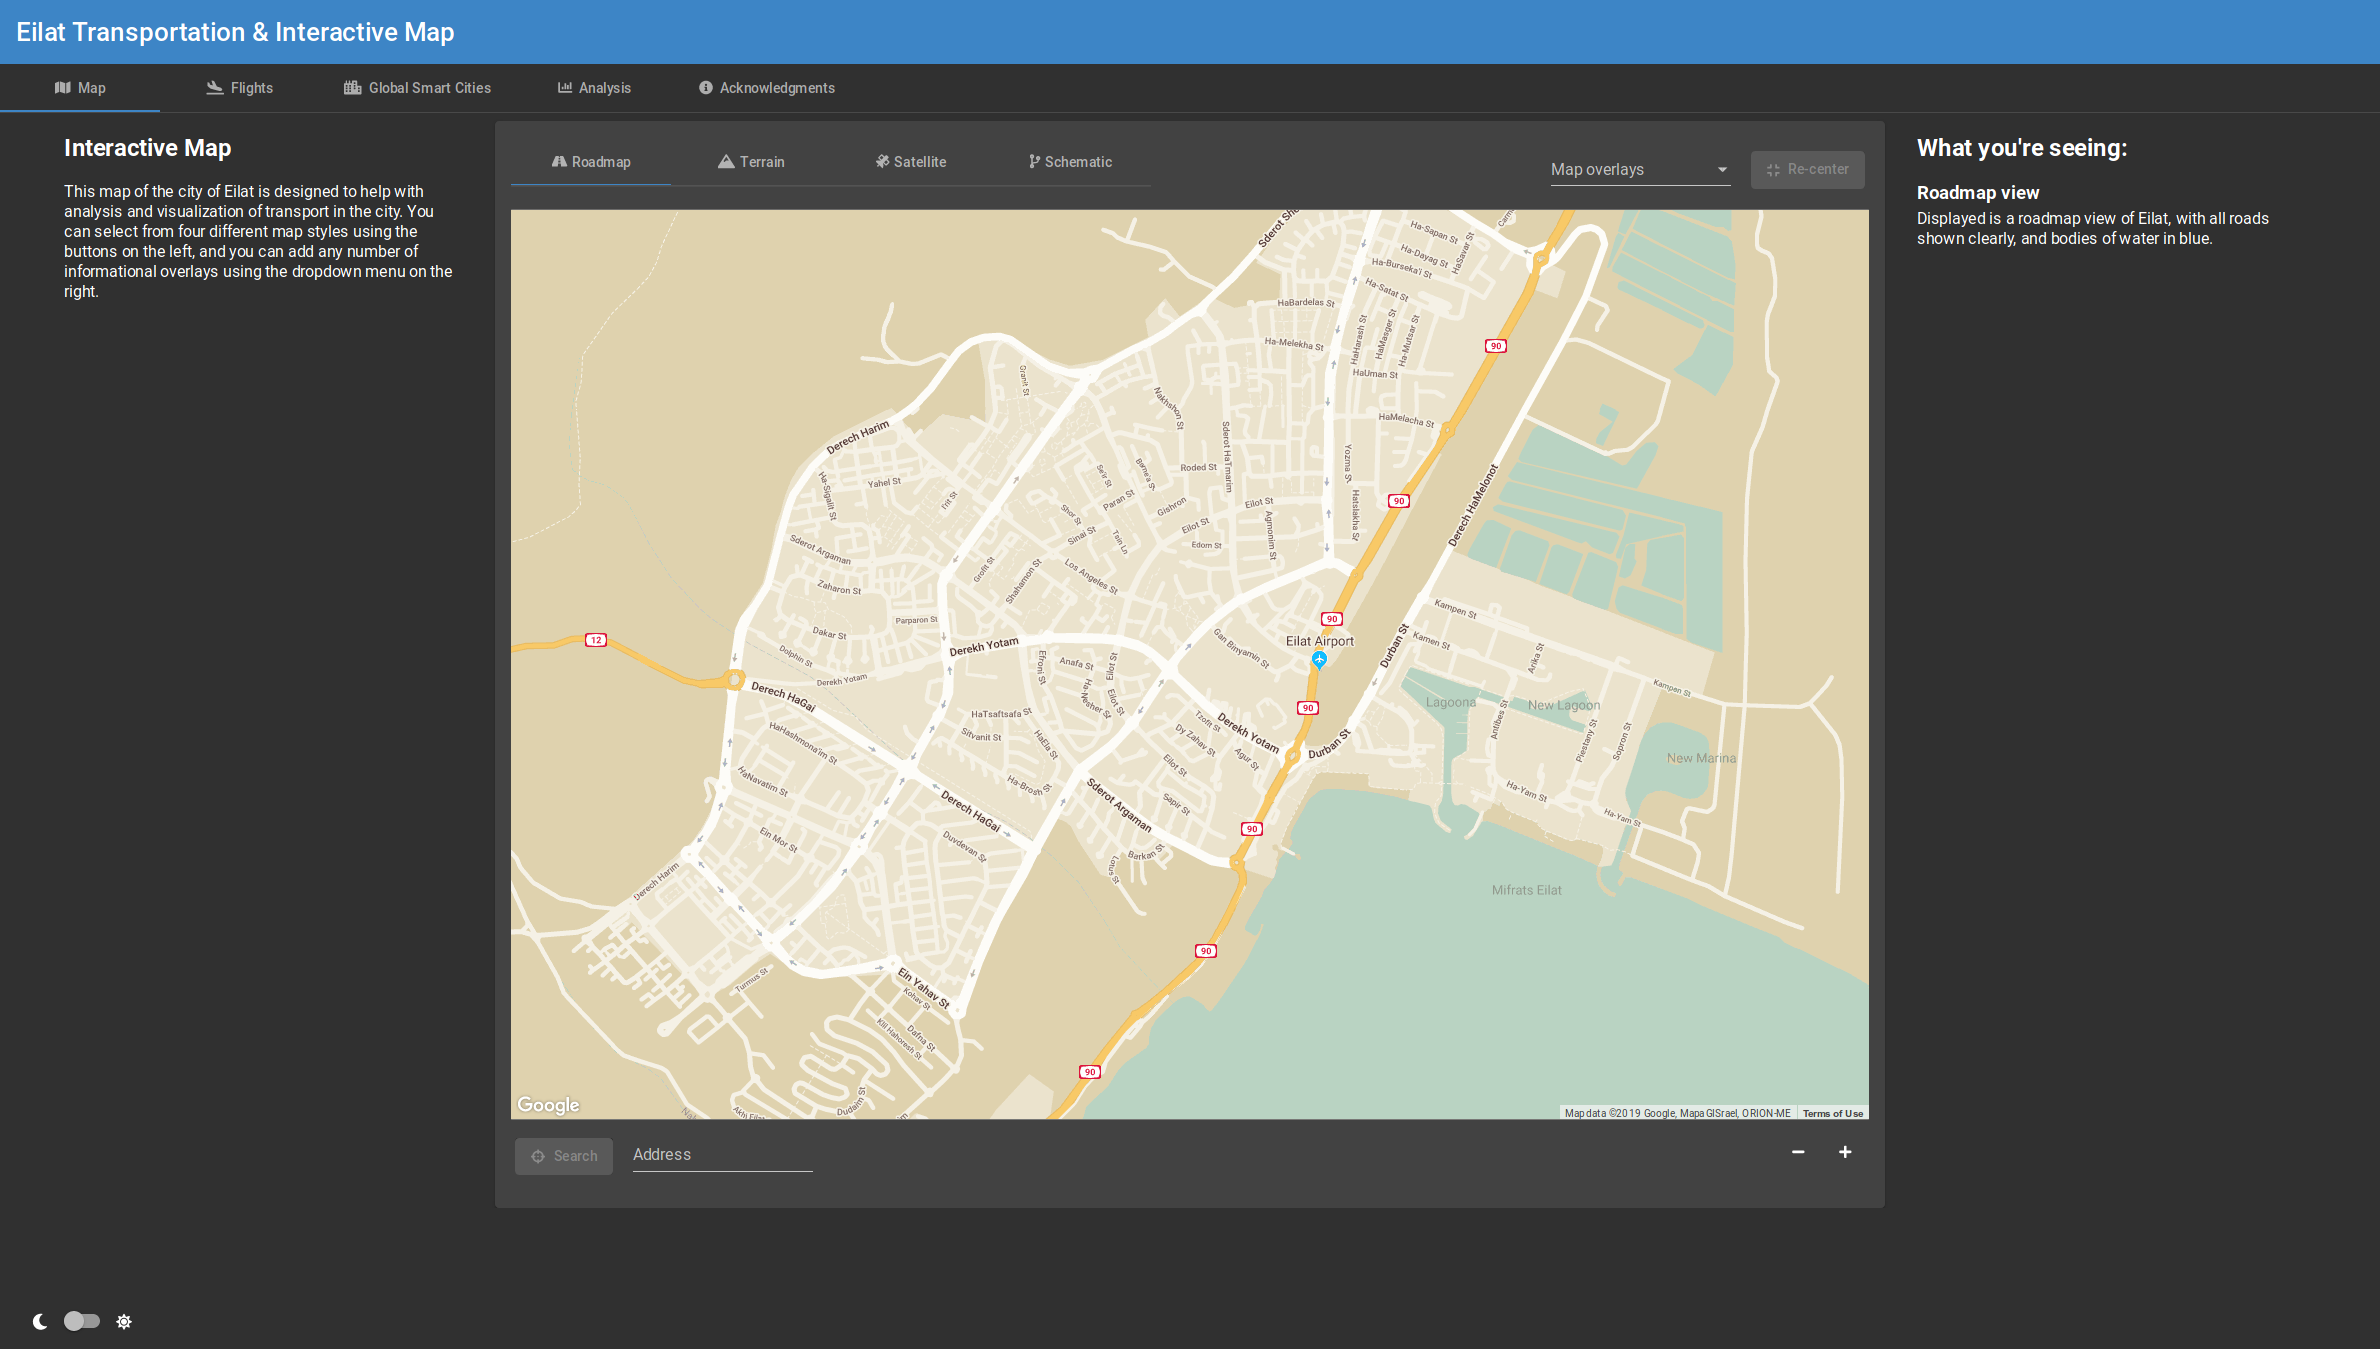
\includegraphics[width=12cm]{images/site_map.png}
    \caption{Website default map view}
    \label{img:site_map}
\end{figure}

Figure \ref{img:site_map} shows the website when it first loads and the default map view, as generated by Google Maps. The left and right columns explain the purpose of the map and any features that might be visible. Four map view modes are available: traditional roadmap view, terrain view (for understanding the effect of geography on the city), satellite imagery view, and schematic view.

\newpage %TODO: REMOVE \newpages AS NEEDED
\begin{figure}[H]
    \centering
    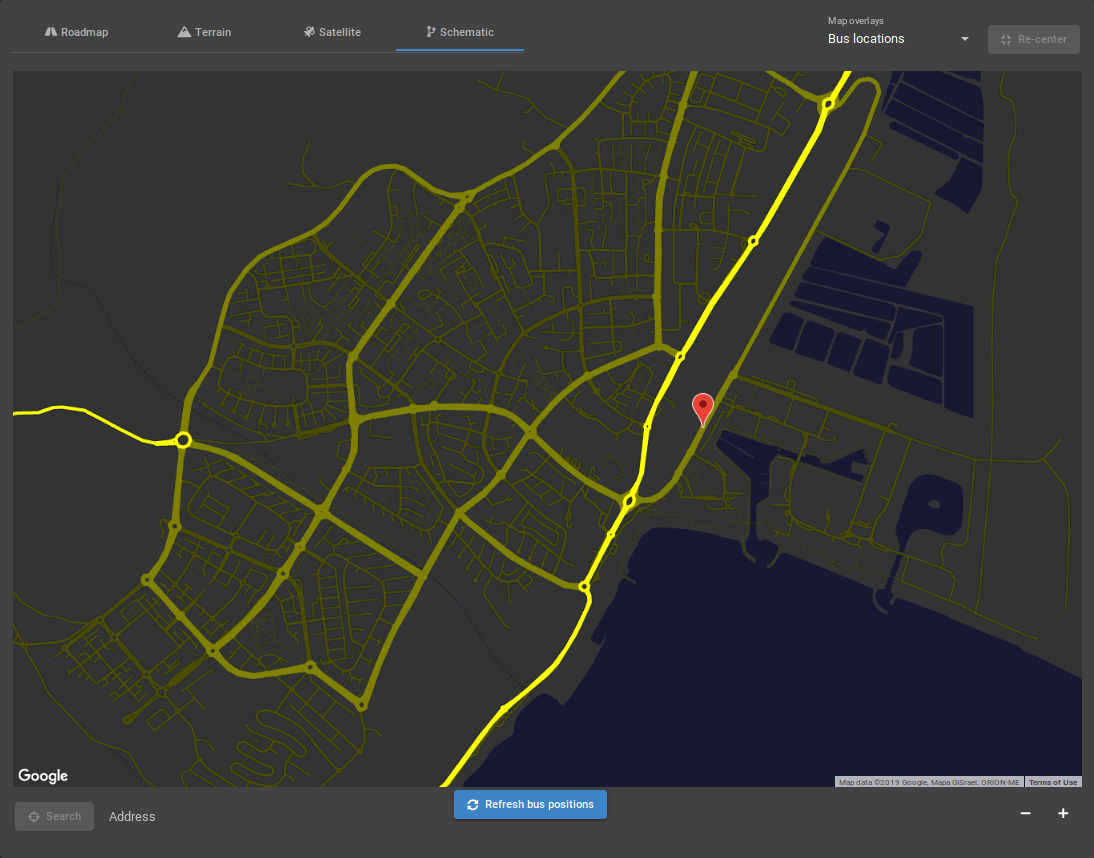
\includegraphics[width=12cm]{images/site_map_schematic.png}
    \caption{Map schematic view with bus location markers} 
    \label{img:site_map_schematic}
\end{figure}

The "schematic view" in figure \ref{img:site_map_schematic} can be used to highlight road size using color; bright yellow lines indicate highways, darker lines are major cities arteries, and the darkest are for local roads. Any number of data overlays can be applied to a map type, such as bus location markers.

\newpage
\begin{figure}[H]
    \centering
    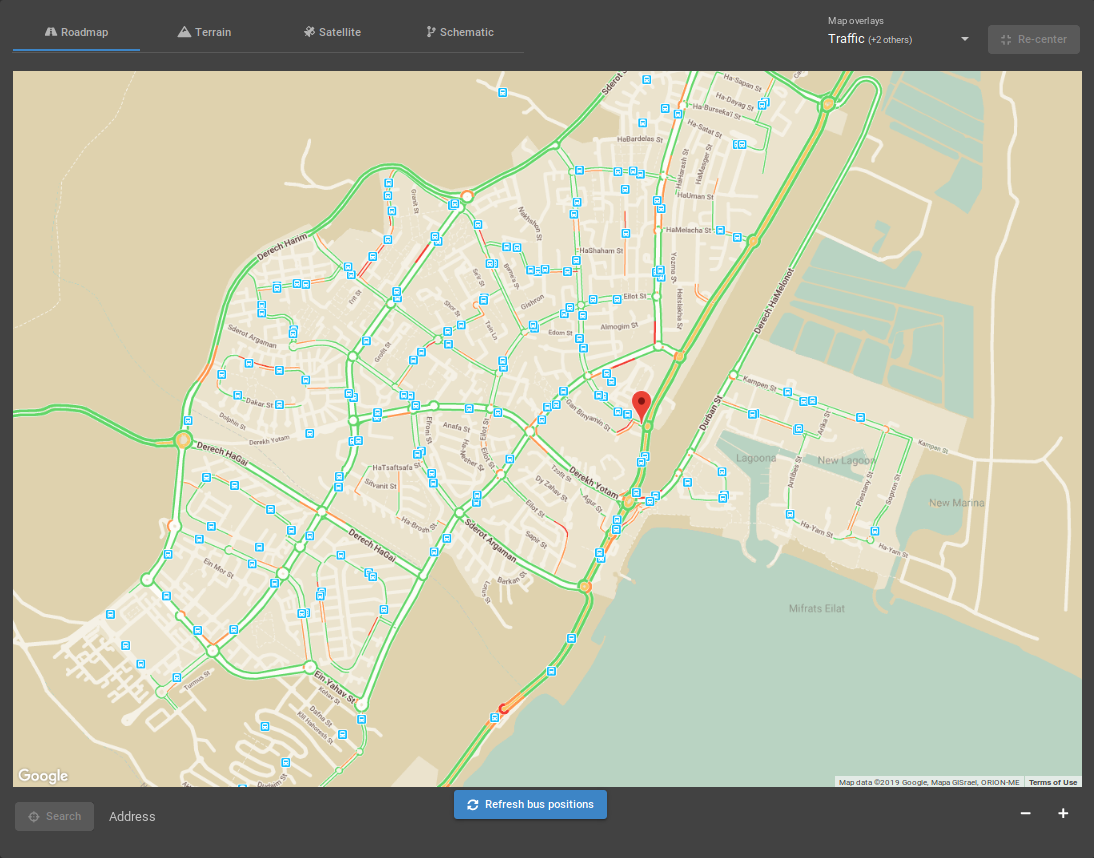
\includegraphics[width=12cm]{images/site_map_traffic.png}
    \caption{Map view with traffic and bus location markers}
    \label{img:site_map_traffic}
\end{figure}

The view in figure \ref{img:site_map_traffic} shows live traffic data alongside locations of buses within the city (\textit{note: this image was taken on a Friday night as services in Israel begin to shut down, so there is only one bus in the city}), which can aid city planners both in understanding where traffic hotspots lie and in understanding how buses interact with traffic. Typically there are 10-12 buses in the city at any given time, many of them clustered together or spending long periods in areas of heavy traffic.

\newpage
\begin{figure}[H]
    \centering
    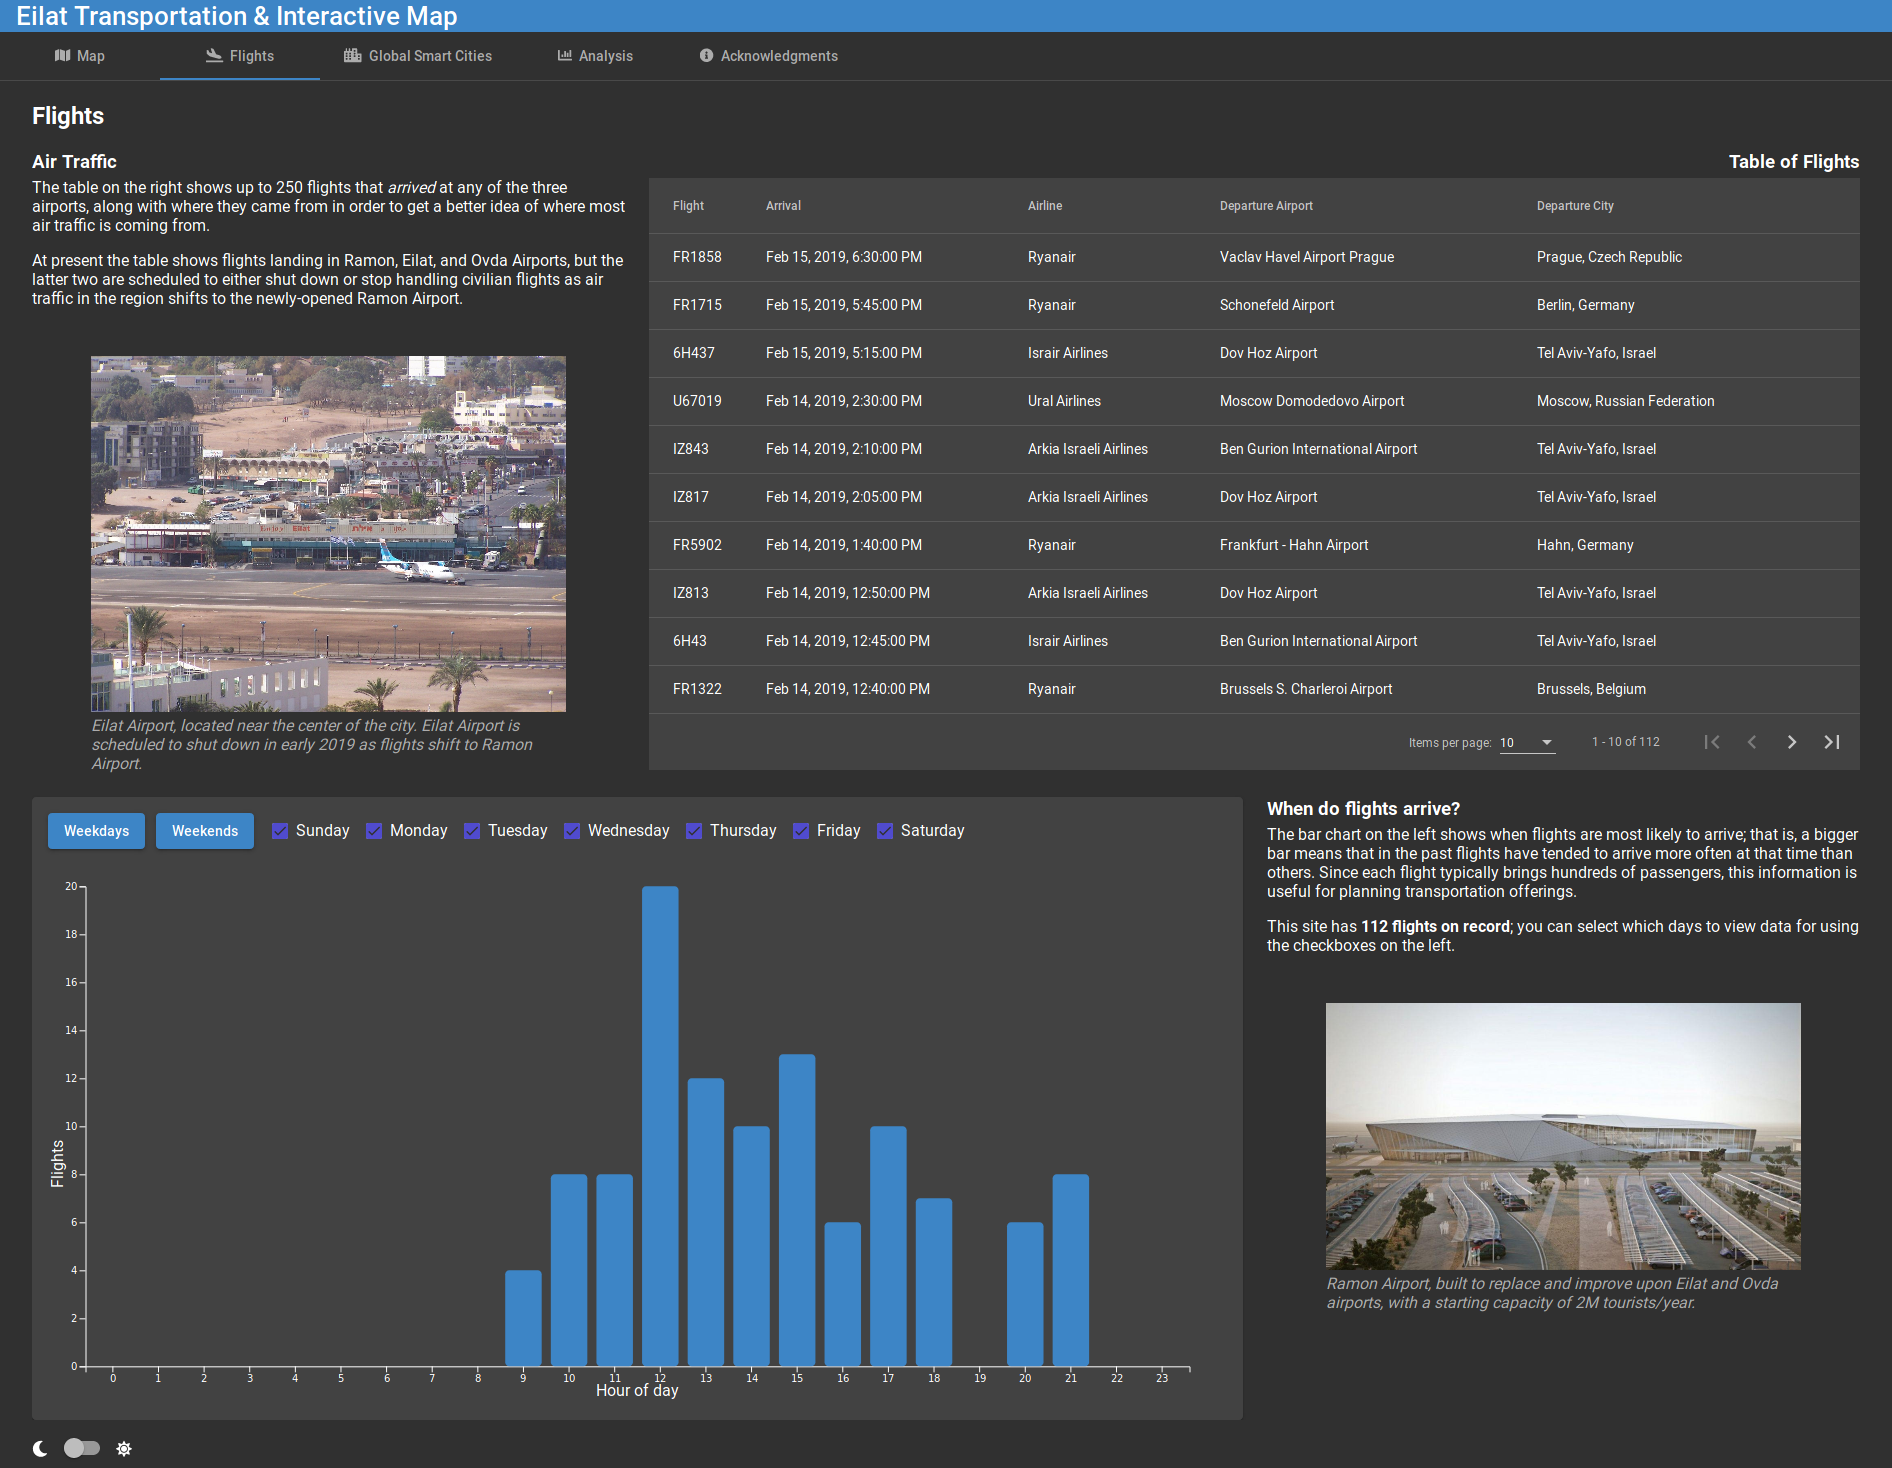
\includegraphics[width=12cm]{images/site_flights.png}
    \caption{Website flights page}
    \label{img:site_flights}
\end{figure}

Figure \ref{img:site_flights} shows the flight data page, built using data on when flights arrive in Ramon, Eilat, and Ovda airports, despite that the latter two are scheduled to effectively shut down as Ramon takes over for air traffic in the region. The chart on the the top right shows a table of the last 250 flights into the region (useful to understand where tourists are coming from), while the histogram on the bottom left (figure \ref{img:site_flights_histograpm}) shows flight arrival times. The table can be sorted by any of its headers, allowing users to quickly search for arrival times, airlines, departure locations, and so on.

\newpage
\begin{figure}[H]
    \centering
    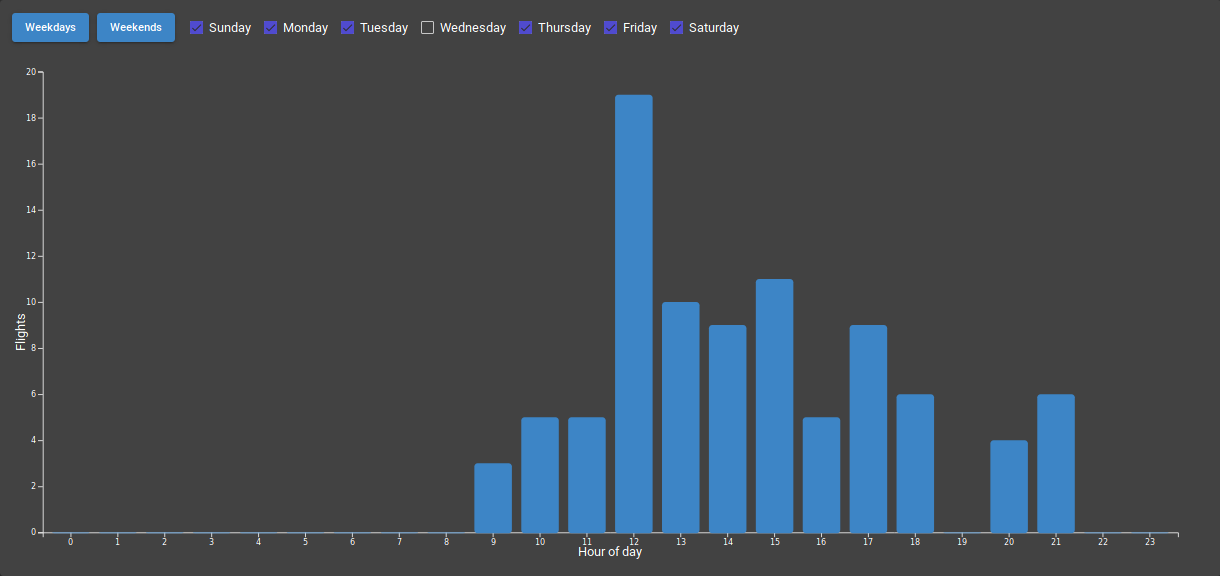
\includegraphics[width=13cm]{images/site_flights_graph.png}
    \caption{Flight arrivals histogram}
    \label{img:site_flights_histograpm}
\end{figure}

The histogram is a fully interactive chart designed to show when flights are most likely to arrive. The higher the bar on the chart, the more flights that have landed in the Eilat region at that time in the past, and thus the more likely it is that flights will land at that time in the future. Since airport traffic may vary by days, checkboxes can be used to select display of data for only certain days of the week. These can easily be toggled in groups using the "weekdays" and "weekends" buttons, which are included since air traffic on weekends is different than air traffic on weekdays.

% This part *probably* isn't needed, but what the hell. Someone feel free to delete it if you want.
\begin{figure}[H]
    \centering
    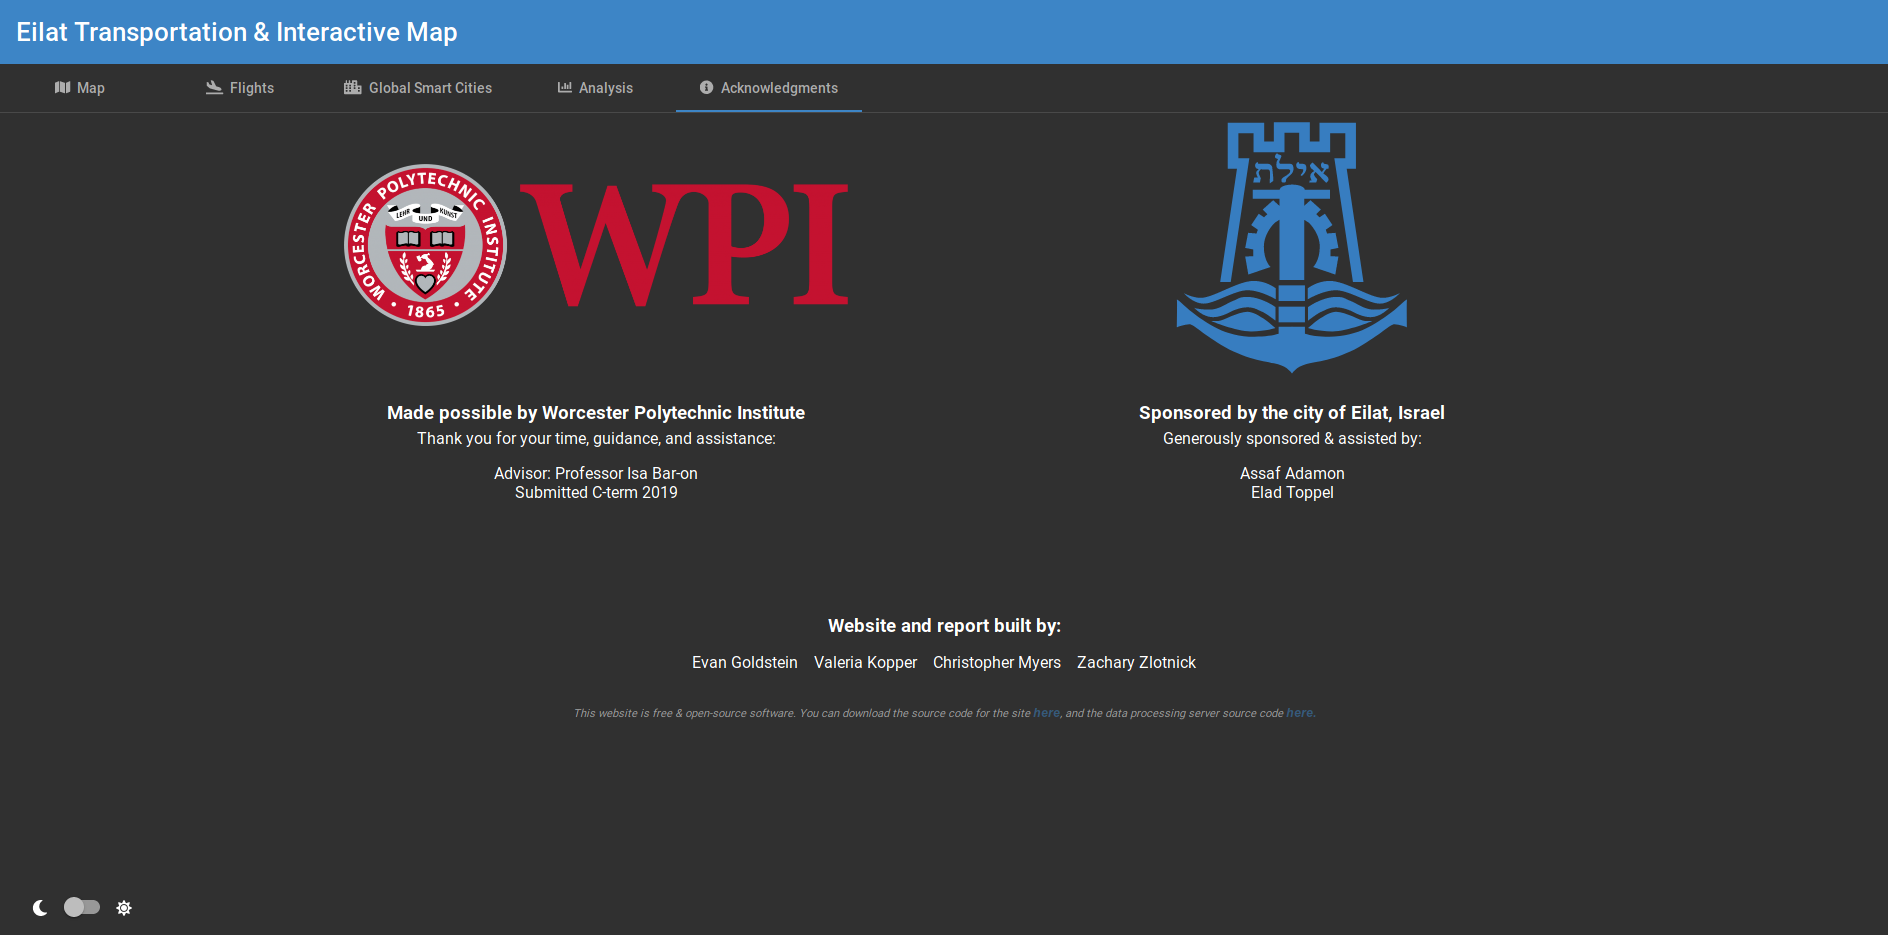
\includegraphics[width=13cm]{images/site_about.png}
    \caption{Website acknowledgments page}
    \label{img:site_about}
\end{figure}

Finally, figure \ref{img:site_about} shows the site's acknowledgments page, which thanks WPI and our sponsors for their time and assistance.

\subsection{Implementation Details}[C.M.]
The website is structured into two components: the front-end website itself (shown in the website overview section), and the data server responsible for processing data and sending it to users of the site for display. The source code for the site is freely available \underline{\href{https://github.com/c7c8/Eilat-Transport-Map-Site}{here}} and the server code is freely available \underline{\href{https://github.com/c7c8/Eilat-Transport-Map-Server}{here}}. Both are designed to operate reasonably independently from each other: the site can receive data from any source, and the data server will provide data to any application.

\subsubsection{Website}[C.M.]
The website is built using the Angular 7 framework to manage data, user interaction, and render the site. Each page is built as its own module, operating independently from the others, making the site much easier to understand and expand, should a future IQP continue development of it. The website uses Angular Material, a library of user interface elements and styles aimed at implementing Google's "Material" design language \cite{2019AngularMaterial}. As a result the site is easy to use, accessible, touchscreen-friendly, and incorporates design elements and behaviors that should be familiar to most users.

The mapping portion of the website is built on top of the Google Maps API, provided as part of the Google Cloud Platform. The API allows display and styling of maps as provided by Google, geocoding addresses to coordinates (this is how the map "search" feature is implemented), and more beyond simple maps of the city. In particular the service allows for the display of overlays and arbitrary datapoints; this is how the traffic overlay is implemented, or how the map is able to display markers to indicate the location of buses within the city. Unfortunately this service is not without cost. The map is unable to display \textit{historical} traffic data as Google simply does not supply it, and requires an API key (to access to the API) to function. API keys can be generated using the Google Cloud Platform console and will not incur any cost, but must be provided by the sponsor in the event they make a clone of the website. The website is alsofully configurable and can be made to source data from any server. This makes it trivial for the sponsor to set up duplicates of the site as needed.

\subsubsection{Data server}[E.G., C.M.]
The data server was written in Python 3 using the Flask server microframework, both chosen for rapid development, minimal up-front requirements, and light footprint. The server provides a small API to request data on three things: the most recent 250 flights landing near Eilat, a data analysis on when those flights land, and the locations of all buses within the city.

Flight data is provided by the \underline{\href{https://www.flightstats.com/v2/}{FlightStats API}} from FlightGlobal, which allows a lookup of all flights arriving at an airport over a period of six hours in only one API request. Just as the Google Maps API requires a key, so does the FlightStats API, but in a more limited sense. This server has been built on top of a trial account that limits the user to 1,000 requests per month, after which requests must be paid for. Consequently the server is set up to retrieve flight data once every 6 hours exactly, store it in a MySQL database for later analysis, and deliver to the website on demand. When the 1,000 trial requests run out, the server will no longer be able to retrieve new data with the same key but will still be able to serve cached data. Similar to the website, the server is also fully configurable and can be set to use any API key and MySQL database.

To analyze data on when flights land, flights are counted by hour and slotted appropriately into a 7x24 matrix (7 days per week, 24 hours per day). The data is then sent off to the site for display on the histogram.

The data server retrieves public transportation information from two sources: the Service Interface for Real-time Information (SIRI) API (specifically the SIRI Stop Monitoring (SM) service) and General Transit Feed Specification (GTFS); both are provided by Israel's Ministry of Transportation. SIRI SM provides real-time information on bus stops, the estimated arrival times of buses at each stop during a given timeframe, and the current location of those buses. GTFS provides static information on public transportation, including bus stop information, scheduled stop times, and bus companies. The GTFS information is stored in the MySQL database and bus stops in Eilat are retrieved by filtering all bus stops in Israel by longitude and latitude. The ID numbers of the bus stops are fed into SIRI SM. From the SIRI response we get the location of all buses currently in Eilat.

\newpage
\section{Conclusion: Suggested Improvements \& Goals}
\subsection{Addressing Congestion}[V.K.]
Currently, Eilat's major transportation problem is highly congested roads, which can be attributed to several factors. These can be mostly encompassed by addressing the current inefficient bus system, the high private vehicle usage, and the lack of alternative modes of transportation. In order to decrease congestion these all need to be improved upon, which demands the creation of goals for Eilat to focus from now to 2040. Goals for Eilat should be based on the data gathered and analyzed regarding Eilat's current situation, the determined problems and influencing factors, as well as the models and goals proposed by case study cities. These goals should serve to identify the gap between Eilat's current situation and where it aims to be by 2040. Establishing the existing gap allows for the identification of the services needed to address each causing factor and goal in order to improve it. This can be majorly separated into three goals: improving transportation and its availability, decreasing private vehicle usage,  establishing mobility as a service. 

\subsection{Improve Public Transportation and Availability}[V.K.]
There are certain goals that can be established as a tangible measurements of improving public transportation in Eilat and its availability by 2040, such as the following: Be within 300-500 meters or within a 5-7 minute walk of a bus stop from any point within the city; limit wait time at a bus stop to 10-15 minutes; decrease travel time, once on the bus, to 20 minutes from point A to point B (anywhere within the city); increase the percentage of population that uses public transportation, both residents and tourists.

In order to increase the percentage of the population (including tourists) that uses public transportation there is a need for investment and improvement of the bus system. This requires the addition of more bus stops throughout the city, so that walking to a bus stop can take between 5 to 7 minutes from anywhere in the city. For more efficiency there should be more buses designated to intra-city transportation. Additionally, existing bus routes should be reevaluated and changed to reflect traffic congestion and user demand. Bus routes are currently spread throughout the city in an non-efficient manner that leads to long travel times. Changing this to shorter routes that target specific areas in the city and that are repeated more often can help address this.

The implementation of shuttles in addition to the existing bus system is worth considering. For example, there are large residential zones in the western part of the city. During peak times most people tend to commute towards the industrial zone and the hotel zone (due to most jobs being within these two areas). Adding a shuttle system that works during these times to target specific neighbors and take residents to their work area and back would help promote the use of public transportation.
    
If public transportation is more efficient (meaning it takes less time to get from point A to point B) and it is more convenient (in that bus stops are close by and waiting times are short) more people are much more likely to use public transportation as the main form of transportation within the city. By achieving this, the use of private vehicles will significantly decrease, which in turn will majorly aid in alleviating congestion. Installing sensors throughout out the city can allow for smart traffic management which would lead to smoother traffic flow, and therefore quicker bus rides.

Providing a user friendly experience can also be greatly beneficial. This can be accomplished by having an app that allows for digital payment (minimizing interactions and the language barrier with bus drivers). The app can also include real time data provided through sensors in order for bus schedules to reflect update times, which serves to reduce wait times. It should also provide directions as to how to get to the nearest bus stop and directions to your final destination from the nearest bus stop. The app should be offered in languages additional to Hebrew in order to accommodate international tourists. 

\subsection{Decrease Private Vehicle Usage}[C.M.]
A seemingly obvious solution to reducing traffic is to reduce the number of cars in Eilat, or more specifically the number of private vehicles. Naturally this would lead to increased reliance on public transport and therefore fewer cars on the road, decreasing congestion and \textit{increasing} the effectiveness of public transport like buses. This will cause more people to use public transport and get off the road, and so on --- a feedback loop. The same is true in reverse, though (more traffic means ineffective public transport, meaning fewer people using it), so getting cars off the road and promoting public transport will require serious up-front effort and policies until traffic decreases enough.

There are a number of policy options available for getting cars off the road. The most immediate possibility is to provide direct incentives to residents to reduce the number of cars they own, like tax breaks for having one car or less per household, tax write-offs for using public transport, or penalties for owning more than one car. To make carpooling more attractive, lanes could be marked as allowing only vehicles with more than a set number of people in their car. Another possibility is to require payment for parking (ex. parking meters) in a progressive fashion that increases as you approach the city center or other designated zones, discouraging people from driving through high-traffic zones to their final destination. Discounts could also be applied to those who choose to carpool, further helping to remove cars from the road. For more policy examples, see \S\ref{sec:policies}.

As for policies aimed at Eilat's tourists, improved public transportation is likely the best overall solution, depending on how tourists tend to get into the city. Those who fly or take buses into the city are more suggestible to using other transport than those who drive, so policies should be aimed at the two groups independently. Someone who didn't drive to Eilat should be made readily able to explore the city without renting a car or calling a taxi, meaning fast and cheap transport from Eilat's hotels is a must. On the other hand, someone \textit{with} their own car must be incentivized to leave it behind, and won't be affected by tax breaks or penalties like an Eilat resident would. Affordable parking outside main areas of the city combined with effective public transport is likely the best way to convince them to leave their cars behind.

\subsection{Establish Mobility as a Service}[Z.Z.]    
It is important to note that the previously mentioned reduction in private vehicle usage should result in an uptick in the use of provided mobility services. The definition of an effective service can vary based on the associated price, convenience, reliability, weather, safety, or travel time. In order to detach citizens in Eilat from their steering wheel, services across the board will need to focus on addressing the gaps existing services exhibit in accordance to these factors. 

The variance in demographics will make the selection of services that reflect the individualized needs of cities significantly more difficult in comparison to other popular destinations. For example, cities like London, Bankok, and Paris were the three most popular tourist destinations of 2018; however, if you at the tourist per capita ratio (tourists to residents), only Paris exceeded Eilat. Both London and Bankok were well under 3 compared to Eilat's ratio of 5, with Paris being about 9 \cite{Murray2018MostInsider}. This means that, especially at times of peak tourism during the summer, the services need to reorient themselves toward the average tourist: typically someone with less than average knowledge of the existing system, who is willing to spend a reasonable amount, and may not speak Hebrew. Taking this into account, effective services for tourists will need to provide ease-of-use before anything else. In contrast, one of Eilat's 50,000 residents would likely prefer to see minimized travel times in junction with a minimized price. 

Ensuring accessible and affordable transportation are two goals for the services which should embody the consumer values above. In order to gauge the accessibility, the city can measure via surveys or tests the viability of getting from one point to another only 10 minutes slower than if they used their own private vehicle. This time should be measured from parking spot A to parking spot B for private vehicles, and will vary during times of peak congestion and/or peak tourism seasons. This goal would primarily interest Eilat residents the most, since they struggle morning and afternoon getting to and from work. For tourists, accessibility should be provided through an app interface which specifically targets the language and payment barriers. This includes providing routing information with associated stops and linked wayfinding apps for the "last mile."

Affordable transportation should be fairly similar for both parties. Currently, bus prices within Israel are extremely reasonable which is one of the largest advantages over other methods of transportation within Eilat. Taxi services are at a predetermined variable cost, in that riders are informed that their rides will be contingent on the traffic at the time and the distance. Keeping customers informed ahead of time what these costs are, similar to Uber and Lyft, would likely garner more users and be more desirable for tourists familiar with those services. This is entirely realistic given that taxi drivers often make up fares on the spot when riders fail to use the Gett app, and riders would feel less taken advantage of.

\subsection{Implementations}[V.K.]
The city of Eilat should invest in the infrastructure necessary for the proposed improvements and technologies. Sensors, cameras, and WiFi should be installed throughout the city to monitor and control parking, traffic lights and street lights, and smart public transit (\S\ref{sec:smart_city_sensors}). Collected data from these should be shared through an open data platform. Services should be tailored to Eilat and some of the most useful ones in establishing mobility as a service are the following: a shuttle system, bike-sharing and car-sharing, car e-rentals, last mile solutions (such as e-scooters, an app for buses (\S\ref{sec:smart_city_services}), and biking lanes. The possibility of a well-established pedestrian center and/or the expansion of the existing boardwalk would also be recommended. 

%Apps should be developed to allow prepaying for public transit services, and should be available in multiple languages. Ideally, a single app would include options for buses, taxis/ride-sharing services, as well as last-mile solutions such as bikes and scooters.

% - Reorganized hours for certain services
% 	=> delivery/school/airport peak hours
% - Address the issues the bus ain't doing for the city rn

\subsection{Sustainability Considerations}[V.K.]
Smart city technologies largely encourage sustainability considerations. Installed sensors can also be used for street light controls and public water usage, such as in parks (\S\ref{sec:smart_city_sensors}). Cameras can also be used to monitor the city's cleanliness. Installing EV charging stations throughout the city can promote EV use, thus further encouraging sustainability initiatives within Eilat. 

\subsection{Summary}[C.M]
The goals above are intended to guide Eilat over the next 20 years and are flexible, but there are some clear elements Eilat should strive for. Eilat needs to improve its public transport offerings to be more efficient, faster, and friendlier for the residents and tourists alike --- quality of offerings can be easily gauged by the percentage of the population using public transport. Offerings should be smartly managed and information should be both collected and delivered to users electronically. At a policy level the city should consider perks for going carless or carpooling, and penalties for those who drive in excess, but not impinge on quality of life and city accessibility. Finally, the city should be open to exploring pedestrian and mobility-as-a-service options to further reduce traffic and environmental impacts, while taking into consideration Eilat's climate and expansion plans.

% * Discuss the goals above and how to realistically measure them in the near future. Determine possible metrics for measure "good" prices, and "good" times.  
% Quality of life
% Prioritize pedestrians and cyclists

% Bibliography -- automatically managed in APA style, on a new page
\newpage
\bibliographystyle{apacite}
\bibliography{refs}

\end{document}